\section*{The Self Replicator Model} 
We begin by presenting a complete derivation of the self-replicator model 
of bacterial growth. We follow a similar approach taken by others 
\cite{scott2010, scott2014, klumpp2013} but without reliance on empirical measurements 
of ribosome content as function of growth rate as a motivating force. Rather, 
we consider the fundamental processes of bacterial growth  as is cartooned in Figure \ref{fig:processes}, formulating intuitive, quantitative 
expressions which capture the dynamics of nutrient consumption to form charged-tRNAs 
and their subsequent consumption to form new proteins.

\begin{figure*}
    \centering{
        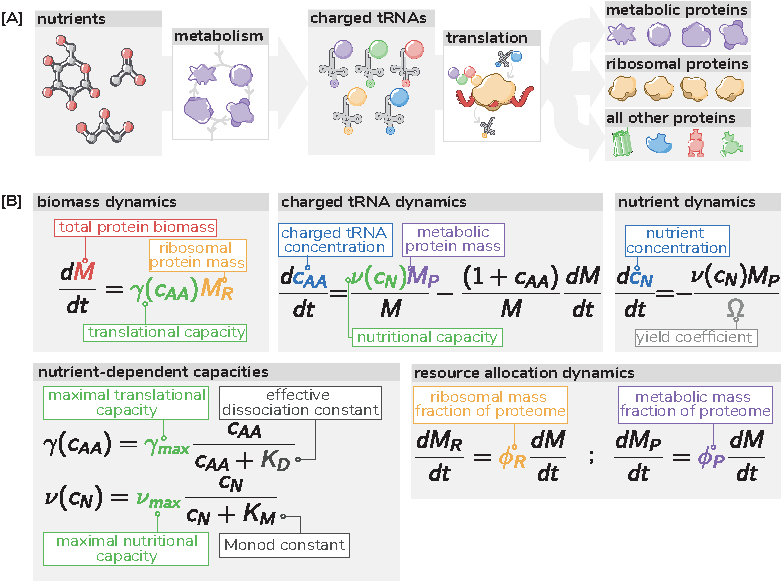
\includegraphics{figures/Fig1_processes_equations.pdf}
        \caption{\textbf{The flow of mass from nutrients to proteins}. [A] The 
        self replicator model describes the consumption of environmental 
        nutrients via the cellular metabolic machinery to produce charged-tRNAs. 
        The subsequent pool of charged-tRNAs are consumed primarily through the 
        process of protein translation via ribosomes to yield new protein biomass 
        partitioned in to metabolic, ribosomal, and "other" sectors. [B] The 
        processes in [A] can be mathematicized to a series of differential equations 
        capturing the dynamics of the mass flow from nutrients to proteins.
    }
    \label{fig:processes}
    }
\end{figure*}

\subsection*{Protein Translation}
We consider a growth regime in which the synthesis of new protein mass $M$ 
is the most resource intensive task of a growing cell. This synthesis results from 
the concerted action of a pool of ribosomes $N_R$, each of with forming new protein 
mass at a rate $k_R$ such that 
\begin{equation}
   \frac{dM}{dt} = k_R N_R. \label{eq:num_ribos} 
\end{equation}
Rather  than explicitly considering the total number of ribosomes in the system, we can 
relate this to the the total ribosomal mass $M_R$ noting that a single ribosome 
as a proteinaceous mass $m_R$, yielding 
\begin{equation}
    \frac{dM}{dt} = \frac{k_R M_R}{m_R} = \gamma M_R. \label{eq:gamma_Mr}
\end{equation}
Here, we have introduced the parameter $\gamma = \frac{k_R}{m_R}$, commonly referred 
to in the literature as the \textit{translational capacity}\cite{scott2010}. This parameter, with 
dimensions of inverse time, represents the fraction of a ribosome's protein mass that 
can be synthesized per unit time. The inverse of this parameter corresponds to the amount of 
time it takes to synthesize the protein components of a single ribosome, which 
for \textit{E. coli} is approximately 7 minutes \cite{dill2011}.

The individual units of protein mass are amino acids, which are supplied to
the elongating ribosome as a charged tRNA molecule. When these are in
abundance, the enzymatic process of forming a new peptide bond becomes the
rate limiting step, yielding a maximal translational capacity $\gamma_{max}$.
However, when charged-tRNA is limiting, the recruitment of charged tRNA to the 
elongating ribosome can become the dominant time scale, reducing the translational capacity 
from its maximal value. These time scales can be related mathematically as 
\begin{equation}
   \frac{1}{\gamma} = \frac{1}{\gamma_{max}} + \frac{1}{k_{on} c_{AA}} \label{eq:timescales} 
\end{equation}

where $c_{AA}$ denotes the concentration of the charged tRNAs present in the cell 
and $k_{on}$ is the effective on rate of the charged tRNA to the A-site 
of the ribosome. Equation \ref{eq:timescales} can be rearranged to the form of a 
Michaelis-Menten relation with the effective dissociation constant $K_D = \frac{\gamma_{max}}{k_{on}}$,
\begin{equation}
\gamma(c_{AA}) = \gamma_{max}\frac{c_{AA}}{c_{AA} + K_D}. \label{eq:gamma_caa}
\end{equation}
While we have presented the charged tRNAs as a concentration, it will prove helpful 
for us to think of it rather as the relative abundance of the total charged tRNA mass 
$m_{AA}$ to the total biomass $M$, $c_{AA} = \frac{m_{AA}}{M}$. The mass fraction and 
true concentration are related to one another via an empirical constant and can 
be easily interconverted, as has been demonstrated previously \cite{klumpp2013, scott2014}. 

\subsection*{Production of charged-tRNAs}
In typical laboratory conditions (and in the data we explore later in this work), 
the amino acids attached to the tRNAs must be synthesized \textit{de novo} from 
minimal nutrient sources such as simple sugars and inorganic salts. Thus, for a 
given combination of nutrients, the dynamics of the charged-tRNA concentration $c_{AA}$ 
can be written as competition of production and consumption processes,

\begin{equation}
   \frac{dc_{AA}}{dt} = J_{AA} - \frac{1}{M}\frac{dM}{dt}(1 + c_{AA}). \label{eq:caa_dynamics_flux}
\end{equation}
Here, we denote the production flux of charged-tRNAs from nutrients in units of concentration 
as $J_{AA}$. The consumption of the charged-tRNAs occurs directly from the direct incorporation 
of the charged-tRNAs in the growing biomass as well as by dilution.

The formation of these amino acids is the result of the combined action of a battery of metabolic 
proteins which have a total mass $M_P$. This pool of metabolic proteins includes 
elements such as transporters and enzymes directly involved in the metabolism of the 
nutrient as well as all of the accessory proteins which facilitate the flux of 
material through the pathway. While this represents a large number of biochemical 
reactions, we can generalize that the synthesis of amino acids from this collection 
of proteins proceeds at an effective rate $\nu$, yielding an expression for the 
charged-tRNA influx $J_{AA}$ of 
\begin{equation}
J_{AA} = \nu \frac{M_P}{M}. \label{eq:influx}
\end{equation}

The effective rate $\nu$ is typically referred to as the \textit{nutritional capacity} 
and is unique to a particular environmental condition. It represents the mass of 
charged-tRNA that can be produced per mass of metabolic protein per unit time. For
conditions with "high quality" nutrients, such as glucose as the sole carbon source, 
the nutrient capacity is large. Poor quality nutrients, such as acetate supplemented
growth, have a correspondingly smaller value for the nutritional capacity. 

The nutritional capacity 
$\nu$ is  dependent on the concentration of the nutrients in the environment, $c_N$.
When nutrients are plentiful, their conversion to charged-tRNAs via the metabolic 
pathways operates at a maximal level $\nu_{max}$. However, as the concentration 
dwindles, so too does the nutritional capacity. Using similar logic to our treatment 
of the charged-tRNA concentration dependence of the translational capacity,  the 
nutritional capacity can also be written in the form of a Michaelis-Menten relation,

\begin{equation}
\nu(c_N) = \nu_{max}\frac{c_N}{c_N + K_M}, \label{eq:nu_cN}
\end{equation}

where we have introduced the parameter $K_M$ to represent the Monod constant for 
growth on a given nutrient. As there are myriad steps involved in the conversion of 
a single nutrient to a charged-tRNA, we find it more appropriate to consider the Monod 
constant instead of an effective dissociation constant.  

\subsection*{Consumption of nutrients}
By conservation of mass, the the accumulation of biomass necessitates a
decrease in the nutrient concentration $c_N$. The corresponding dynamics are negatively 
proportional to the the production of charged-tRNAs via metabolism $J_{AA}$ scaled by 
a prefactor
\begin{equation}
\frac{d c_N}{dt} = - \frac{\nu M_P}{\Omega}. \label{eq:yield}
\end{equation}

The parameter $\Omega$, termed the yield coefficient, represents the efficiency 
by which a given concentration of nutrient is converted to concentration of charged-tRNA. A
yield coefficient of $\Omega = 1$ implies that for each mass of nutrient consumed, an equivalent 
mass of charged-tRNA is produced. However yield coefficients are rarely so high and 
are typically $< 1$, even for preferential nutrient sources such as glucose in \textit{E. coli}.

\subsection*{Allocation of resources}
The production of charged-tRNAs from raw nutrients and their incorporation into 
new protein biomass, as detailed in Equations \ref{eq:gamma_Mr} - \ref{eq:yield} 
depend on masses of metabolic $M_P$ and ribosomal $M_R$ proteins, respectively. 
While we have defined how the total biomass $M$ evolves in time, we have not 
defined how the resources are partitioned into the growing pools of $M_P$ and $M_R$.

We note that, while we consider only $M_P$ and $M_R$ as being directly involved 
in the dynamics of biomass production, there are many other proteins $M_O$ that 
are also translated. Considering this accounts for all protein production, 
we can parameterize the masses of each protein class as 
\begin{equation}
\phi_R = \frac{M_R}{M}\,\,;\,\,\phi_P=\frac{M_P}{M}\,\,;\,\,\phi_O = \frac{M_O}{M} \label{eq:mass_frac_definition}
\end{equation}
under the constraint
\begin{equation}
    \phi_R + \phi_P + \phi_O = 1 \label{eq:frac_constraint}. 
\end{equation}

Assuming that the corresponding partitioning 
of mass between these fractions is constant in time for growth on a given nutrient, 
we can state the mass dynamics of each class of proteins as 
\begin{equation}
\frac{dM_R}{dt} = \phi_R \frac{dM}{dt} \,\,;\,\, \frac{dM_P}{dt} = \phi_P \frac{dM}{dt},
\label{eq:phi_dynamics}
\end{equation}
which now provides the final piece in our derivation of the self replicator model.

\subsection*{Assembling the model}
Equations \ref{eq:gamma_Mr} -- \ref{eq:phi_dynamics} provide a 
complete description of the flow of mass from nutrients to proteins as depicted in 
Figure \ref{fig:processes}. In Figure \ref{fig:processes} [B], we present all 
of these equations together with the major parameters defined as appropriate. With 
these equations in hand, we can explore the dynamics they encode by numerically 
integrating them over a range of physiologically meaningful values, such as 
those defined in Figure \ref{fig:integrations}[A]. 

Figure \ref{fig:integrations}[B] shows the result of this integration over a range 
of values for the maximal nutritional capacity $\nu_{max}$. While the allocation 
parameters $\phi_R$ and $\phi_P$ are held constant, varying $\nu_{max}$ is comparable 
to tuning the quality of the growth medium, defining different effective rates at which 
the nutrients are converted into charged-tRNAs. 

It is immediately apparent in Figure \ref{fig:integrations} [B] that there is 
a period of exponential growth (linear region in plots) of biomass. During this phase of growth, 
The translational capacity (Figure \ref{fig:integrations}[C]) reaches a steady-state 
fraction of the maximal value $\gamma_{max}$ whose magnitude depends on the maximal nutritional capacity $\nu_{max}$. This 
is in contrast to the nutritional capacity $\nu$, whose value in this phase is equal to its maximal value,
indicating that the nutrient concentration is not limiting.  During the exponential phase of growth, 
the intracellular abundance of charged-tRNAs ($c_{AA}$, Figure \ref{fig:integrations}[E]) reaches a plateau 
at the steady-state concentration. The magnitude of this concentration is dependent on the 
he nutritional capacity $\nu_{max}$ with larger capacities corresponding to larger 
steady-state charged-tRNA concentrations. This explains the dynamics of the translational 
capacity observed in Figure \ref{fig:integrations}[C] where decreasing maximal nutritional 
capacities result in sub-maximal translational efficiencies.  While a steady-state concentration of 
charged-tRNA is reached during this phase of growth, the nutrient concentration 
(Figure \ref{fig:integrations}[F]) continues to steadily decrease until it rapidly approaches zero.

As the nutrients become limiting, The exponential phase of growth concludes and 
the biomass approaches a saturating bound (plateau in Figure \ref{fig:integrations}[B]).
This point corresponds to a rapid plummet in the intracellular concentration of 
charged-tRNAs to a new steady state value of 0, indicating that the nutrients 
of the growth medium have been exhausted and new biomass can no longer be produced.

\begin{figure}[t!]
    \centering{
        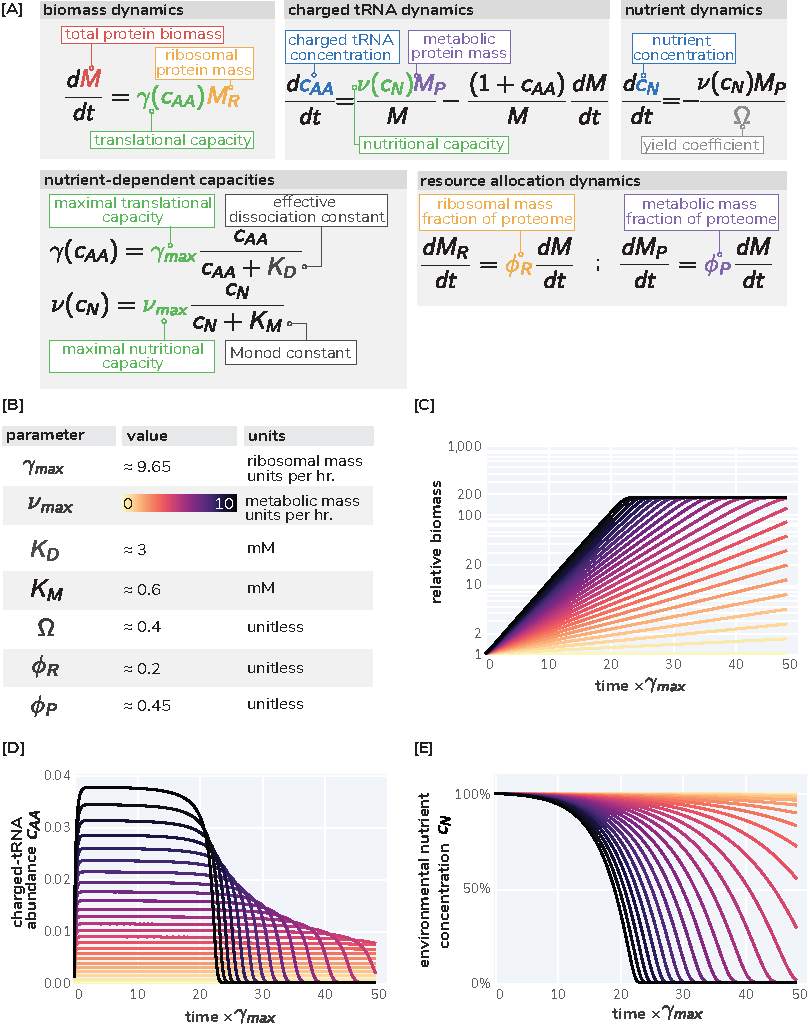
\includegraphics{figures/Fig2_integrated_dynamics.pdf}
        \caption{\textbf{Temporal dynamics of the self replicator model.} [A] Physiologically meaningful ranges 
        of the parameters given literature values of \textit{E. coli} growth 
        physiology {\color{blue}{[GC: note, inlcude BNIDs and add referenences where appropriate]}}.
        The dynamics of [B] the total biomass $M_t$ relative to the initial condition $M_0$, [C] the
        translational capacity $\gamma_t$ relative to the maximum $\gamma_{max}$, 
        [D] the nutritional capacity $\nu_t$ relative to the maximum $\nu_{max}$, 
        [E] the concentration of charged-tRNAs $c_{AA}$,
        and [F] the dynamics of the nutrients in the environment are shown for a 
        range of values for the nutritional capacity $\nu_{max}$.
    }
    \label{fig:integrations}
    }
\end{figure}



